\begin{center}
\begin{tikzpicture}
    \node[anchor=south west,inner sep=0] (image)  at (0,0) {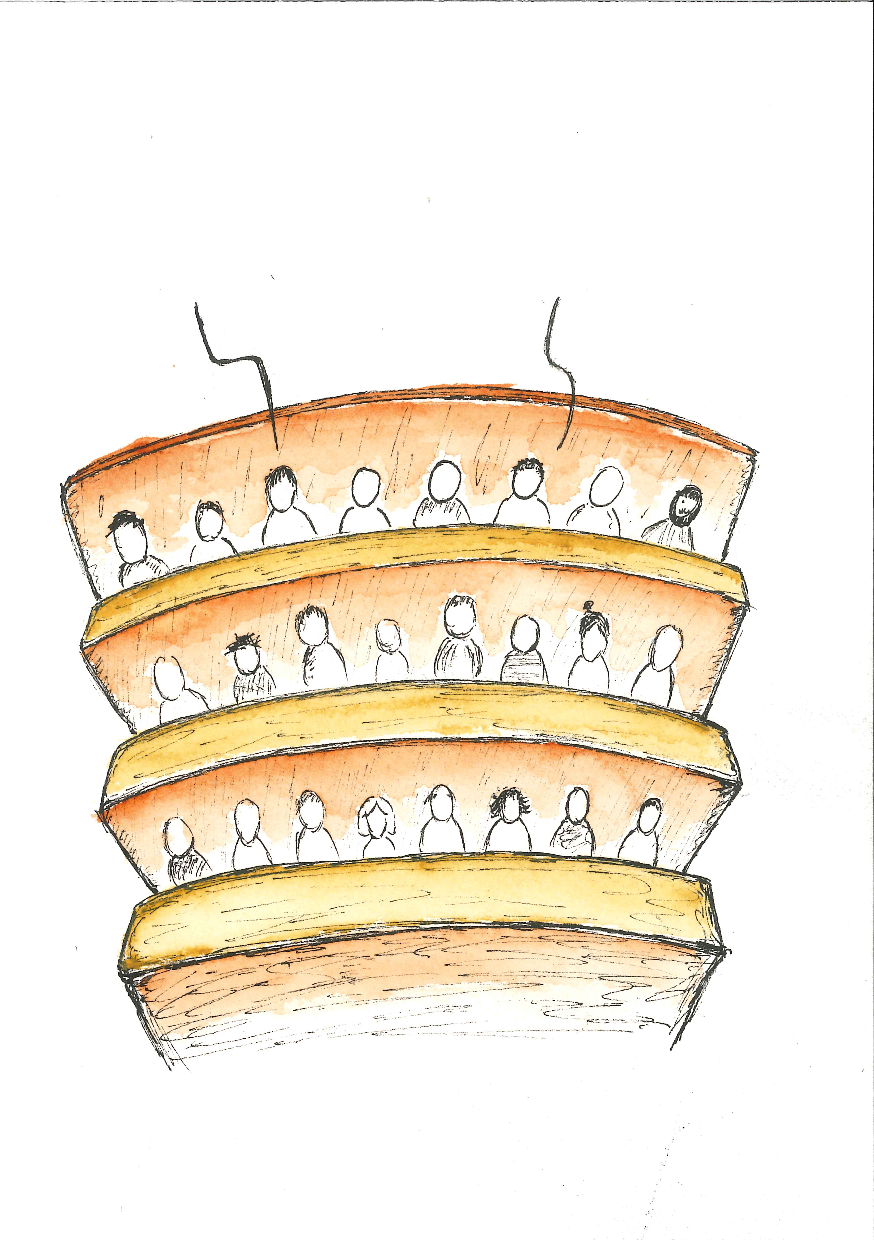
\includegraphics[trim={2mm, 2mm, 2mm, 2mm},width=0.995\pagewidth]{scans/panel-2.pdf}};
    
    
    \begin{scope}[x={(image.south east)},y={(image.north west)}]
        \if\helplines1
        	\draw[help lines,xstep=.1,ystep=.1] (0,0) grid (1,1);
        \fi
        \node[align=center, text width=0.4\pagewidth,anchor=north](en) at (0.7, 0.9) {\english{Excuse me, but why would we care about any of this?
        
        \footnotesize{Will it be on the exam?}}};
        \node[align=center, text width=0.4\pagewidth, anchor=north](es) at (0.21, 0.85) {\spanish{Perdón, pero... ¿por qué nos debe importar nada de esto?
        
        \footnotesize{¿Entra en el examen?}}};
    \end{scope}
    
\end{tikzpicture}
\end{center}